%%%%%%%%%%%%%%%%%%%%%%%%%%%%%%%%%%%%%%%%%%%%%%%%%%%%%%%%%%%%%%%%%%%%%%%%%%%%%%%
%%%%%%%%%%%%%%%%%%%%%%%%%%%%%%%%%%%%%%%%%%%%%%%%%%%%%%%%%%%%%%%%%%%%%%%%%%%%%%%
\chapter{Introduction}
\label{chap:introduction}
%%%%%%%%%%%%%%%%%%%%%%%%%%%%%%%%%%%%%%%%%%%%%%%%%%%%%%%%%%%%%%%%%%%%%%%%%%%%%%%
%%%%%%%%%%%%%%%%%%%%%%%%%%%%%%%%%%%%%%%%%%%%%%%%%%%%%%%%%%%%%%%%%%%%%%%%%%%%%%%

The intent of this dissertation is to document my research into
\emph{formalized score control}\citep{ baca2011xi, baca2015tenor,
trevino2013compositional} in order to demonstrate a \emph{computational model
of music composition}. The term formalized score control, inspired by Iannis
Xenakis' seminal text \emph{Formalized Music}\citep{xenakis1992formalized,
baca2012}, describes the discipline of modeling and manipulating the typography
of common practice notation programmatically via software. An emphasis on
\emph{modeling}, here, is crucial. When working computationally, models provide
an explicit formal description of what objects exist within a given domain, how
they behave, and what transformations they afford. The clearer the model
becomes, the easier it is to extend and to construct increasingly higher-order
abstractions around that model. That is to say, a clear model of notation --
the description of symbols on the page -- affords a clear model of composition
-- how those symbols come to be there.

At the time of this writing, a wide variety of computational models of notation
exist\citep{ baca2015tenor, trevino2013compositional}, expressing an equally
wide range of explicitness or implicitness in their modeling, and providing
composers with varying degrees of programmatic control over those models. For
example, many composers make use of vector graphics programs for notation,
working in a environment which behaves like a hyper-extended writing desk, but
which provides no more semantic understanding of the contents of the page than
a physical pencil does. That is to say, the software make no categorical
distinction between an oval representing a note head and any other line on the
page. Likewise, many composers rely on more traditional notation software which
mimics the physical page while providing some model of common practice
notation, rigidly enforcing a measure-based understanding of musical score on
the artist, while still others make use of the idiosyncratic score-modeling
systems often developed hand-in-hand with computer-assisted composition
tools.\footnote{Composers often make use of all the above categories of tool in
a single score, working programmatically with a computer-assisted composition
tool to generate material which is then exported into a more traditional
notation editor for page layout and further editing, and finally exported as
vector graphics for fine-tuning. This work-flow is not reversible. The changes
made to the score as vector graphics cannot be propagated back into the
semantic model of the score provided by either the traditional score editor or
the computer-assisted composition tool.} Of course it's important to understand
that I don't denigrate the use of vector graphics programs to create scores.
The relative presence or absence of notation modeling in a tool can be a boon
or a hindrance, depending on how it aligns with the needs of the composer using
it. While one tool might model notation exquisitely, it still provides
programmatic control over only what it can describe, and may even forbid the
manipulation of anything beyond that domain. Conversely, another tool,
providing only a minimal model of notation, or even none at all, is not so
constrained, and while it may not afford programmatic control over the contents
of the score at all, it does allow composers to radically reinvent and extend
an understanding of Western notation.

My own compositional work now makes extensive use of the \emph{Abjad API for
Formalized Score Control}.\citep{baca2011xi, baca2015tenor,
trevino2013compositional} Abjad,\footnote{http://projectabjad.org/} which
originated in 2008 as a joint effort between the composers V\'{i}ctor Ad\'{a}n
and Trevor Ba\v{c}a, and to which I have also been contributing significantly
for over six years, extends the
\emph{Python}\citep{vanrossum2003ys}\footnote{http://python.org/} programming
language with a rich model of common practice notation, and visualizes the
scores it models with
\emph{LilyPond}\citep{nienhuys2003ve}\footnote{http://lilypond.org/}, an
automated engraving system inspired by the venerable \LaTeX{}. On top of Abjad,
I have implemented a model of composition in the Python package \emph{Consort},
which allows for the specification of the structure of a score and the
processes to be used to create it, and the interpretation of that specification
first into Abjad's notation model, and subsequently into publication-quality
typography via LilyPond. These twin notational and compositional models bring
the collective knowledge of the computer science discipline to bear on a
variety of musical questions: how does one arrange large-scale form? What
manner of rhythmic, harmonic and timbral transformations are available? How can
one describe formal structural relationships between the objects on a page? How
can one quickly audition and vary dense, multi-layered orchestral textures? The
chapters that follow investigate these two intertwined forms of modeling,
attempting to address some of the musical questions posed here, while paying
special attention to those details -- often missing from treatises on
computer-assisted composition -- which straddle the line between high-level and
low.

Importantly, this dissertation is not a general survey of the techniques used
by composers working in computer-assisted composition, but the work of one
composer implementing for the specifics of his own process. This work may well
be applicable to others in many ways, but I do not claim universality. It is
then, more of a tutorial than anything else, presented in order to explain the
architectural decisions, implementations and implications behind a system
designed to assist in the composition of music.

\section{Background \& Motivation}
\label{sec:background-and-motivation}

Computer-assisted composition has a fairly short history, dating at the time of
this writing a little more than half a century. While one could certainly argue
about the timeline and origins of the techniques falling under this umbrella --
and providing a complete history of computer music is not the goal of this
dissertation -- it is generally agreed that work began in earnest in the
post-war decades of the 20th century.\citep{curtis1996computer,
xenakis1992formalized} Despite its relative youth as a musical tradition,
computer-assisted composition has many practitioners and a tremendous number
of tools to work with, both generalized and idiosyncratic.

My personal introduction to computer-assisted composition began with Iannis
Xenakis' mid-century massed string works,\citep{xenakis1992formalized} and,
combined with a life-long interest in electro-acoustic music dating back to my
serendipitous childhood exposure to a copy of Ivan Tcherepnin's \emph{Flores
Musicales / Five Songs / Sant\={u}r Live!}, quickly progressed through study of
Curtis Roads' granular explorations,\citep{roads2004microsound} Trevor Wishart's
schema for textural transformations,\citep{wishart1996sonic} and Kaaija
Saariaho's analytic orchestrations. While I've turned to other music and other
considerations since reading these texts and listening to these works, they
instilled in me a confidence that \emph{somehow} computation could be useful
for creating the sort of music I wanted to hear but was consistently unable to
write, simply sitting at my desk.\footnote{The jury is still out, but I persist
anyway.}

\begin{figure}[tp]
\begin{centering}
\includegraphics[
    page=1,
    width=\textwidth,
    height=0.9\textheight,
    keepaspectratio,
]{assets/dissertation-score-mbrsi.pdf}
\caption{The first page of \emph{mbrsi} (2006), an unfinished tablature score
for one to twelve string performers. This represents an early attempt of mine
at computationally modeling massed performers with timespans to create an
evolving \enquote{granular} texture. The instructions for the score were
created through a variety of Max/MSP patches which painstakingly converted
noise functions into text files which I then collated into spreadsheets. The
score itself was drawn by hand on size A1 graph paper with Rapidographs.
I completed seventeen of the intended fifty-three pages before stopping for the
sake of my wrists and due a general lack of faith in the project. While still
incomplete, the concerns that motivated this score remain with me.}
\label{fig:mbrsi-score}
\end{centering} 
\end{figure}

My earliest experiments with computer-assisted composition involved Max/MSP,
writing patches to generate tabular data from various noise functions which I
collected into spreadsheets and painstakingly notated by hand. That work
culminated at the end of my undergraduate study in 2006 with the
never-completed score \emph{mbrsi} -- excerpted in \autoref{fig:mbrsi-score},
with one spreadsheet \enquote{source} in \autoref{fig:mbrsi-lh} --, whose
textural fabric of massed strings attempted to crystallize the possibilities I
felt in granular synthesis at the time: a kind of sparkling, nervous energy
hovering between a flame and the strange Bezier-cloud outlined by starling
swarms. Unfortunately, the process of simply notating the piece by hand was
gruelling, and effectively forbade any effort at compositional exploration, let
alone revising. In short, while this early work did take lengths to model a
compositional process, it lacked any notational model beyond my own hands. And
in the absence of any automated typesetting tool, the project collapsed under
its inherent labor difficulties. I set \emph{mbrsi} aside and spent the next
few years looking for alternative approaches to both formalizing large-scale
structure in score, and automating the typesetting of those structures into
notation, going so far as to attempt scripting various vector graphics programs
directly in order to establish a formalized model of music notation which
I could use to complete the project.

\begin{figure}[tp]
\begin{centering}
\noindent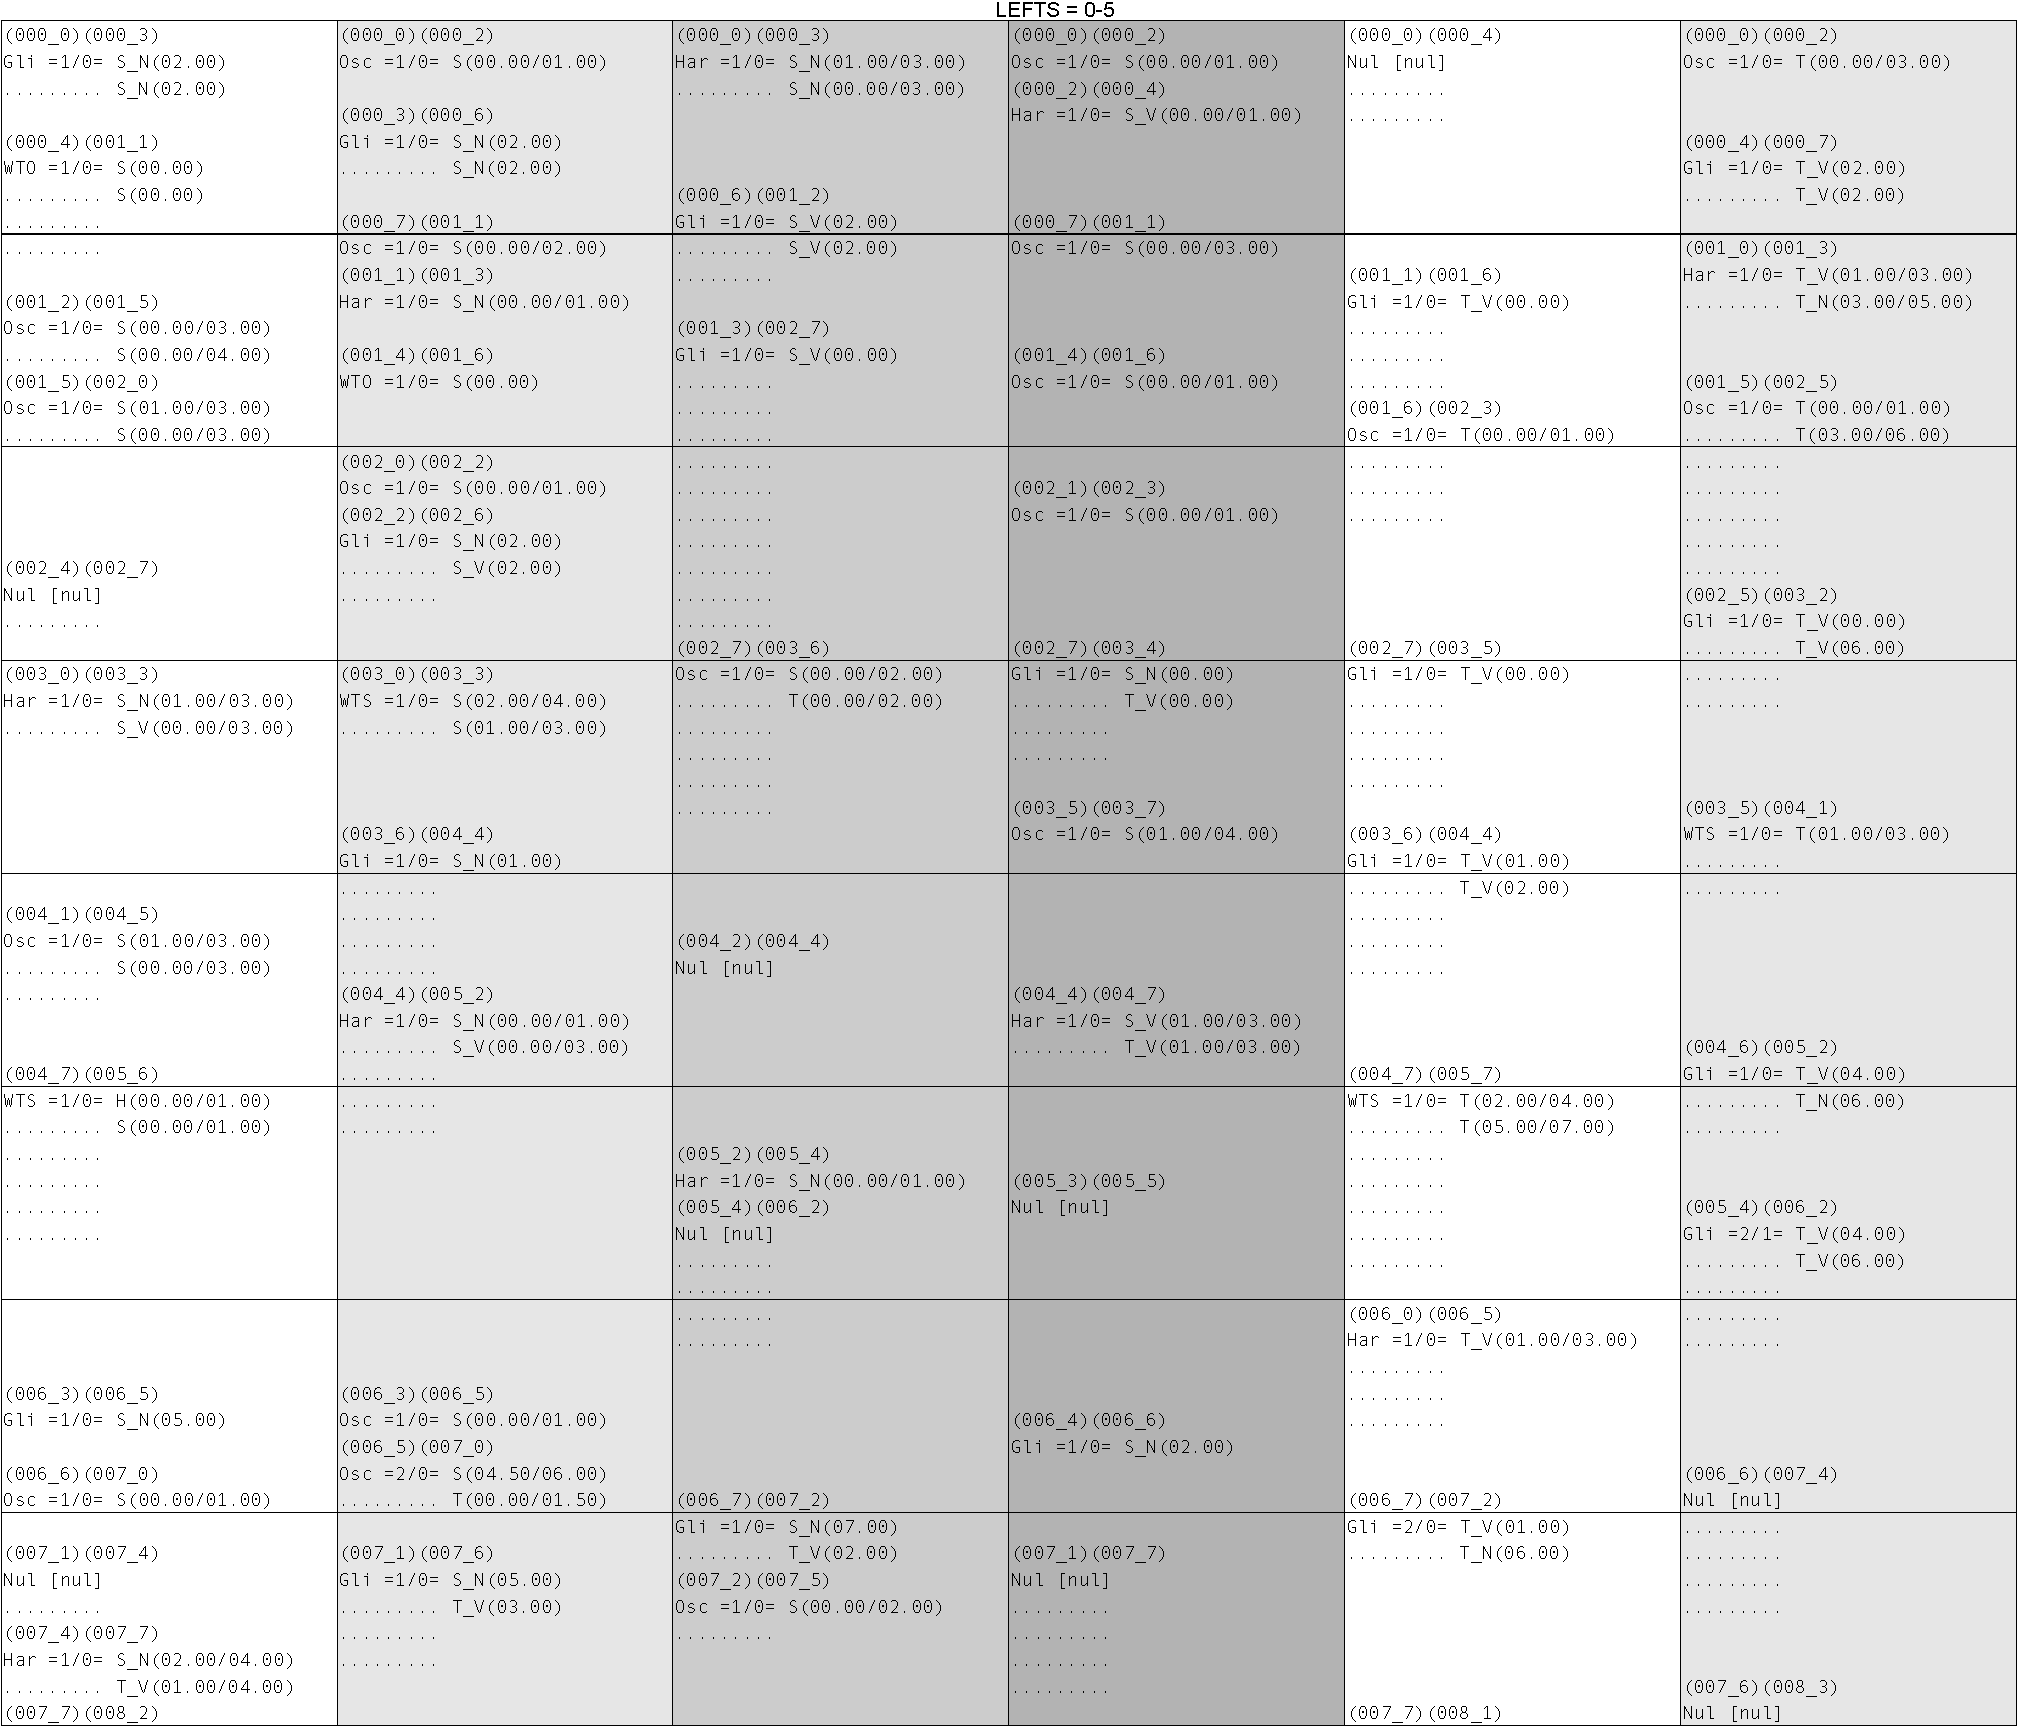
\includegraphics[
    clip=true,
    trim=0in 0in 0in 0.125in,
    page=1,
    width=\textwidth,
]{assets/dissertation-score-mbrsi-lh.pdf}
\caption{Page one of fifty-three from a spreadsheet containing fingering
instructions for six of the twelve string performers in \emph{mbrsi} (2006).
Each box consists of the instructions for one performer, over the course of one
measure. The instructions in the upper-left box here correspond to the
upper-most row of boxes in \autoref{fig:mbrsi-score}.}
\label{fig:mbrsi-lh}
\end{centering} \end{figure}

%Some of the most important tools available contemporary with my entry into the
%field include OpenMusic, PWGL, Common Lisp music, and somewhat later the BACH
%library for use with modern versions of Max, as well as a whole host of more
%marginal experiments including LilyCollider which provides an interface between
%SuperCollider -- generally used for live electronics -- and LilyPond.

\todo[inline]{Mention OpenMusic, PWGL, Common Lisp, BACH, etc.}

A number of years later, at the beginning of my graduate studies, I was
introduced to first LilyPond, and then Abjad. LilyPond, much like \LaTeX{},
is a command-line tool takes a text file comprising various commands which
describe the content of a musical document, and converts those commands into
graphic representations of music notation, generally as a PDF. This working
modality is often referred to as \enquote{what you see is what you mean}: the
user of the system edits with the intent to describe their desired structure,
rather than manipulating a representation of the end-product itself. The
discovery of a such a plain-text-based way of working was a revelation to me,
precisely because plain text is eminently susceptible to manipulation. One
would be hard-pressed to find \emph{any} programming languages which cannot
generate plain-text files. While hardly easy -- and I simply couldn't have
known at the time how far off that impression was -- a way forward finally
seemed possible: I could develop a system to model notation, using LilyPond as
its typesetting engine. Luckily, V\'{i}ctor Ad\'{a}n and Trevor Ba\v{c}a had
reached an identical conclusion sometime before, and had already begun the work
of implementing a notation model in the Python programming language, using
LilyPond as the primary output.

\vspace*{0.25\baselineskip}
\todo[inline]{Fill in the intervening years.}
\todo[inline]{Why are other systems unnecessary?}

\section{Overview of the dissertation}
\label{sec:overview-of-the-dissertation}

This dissertation consists of six chapters of prose -- including this chapter
--, followed by five chapters each presenting a score, and four extensive
appendices comprising complete code listings for the implementations of the
three most recent scores and of Consort. Please consult the source for Abjad
version 2.16\footnote{https://github.com/Abjad/abjad/releases/tag/2.16}
directly, as it is far too large to include here.

The first six chapters discuss formalized score control, gradually laying out
and building upon the concepts necessary to understand the process of modeling
notation and composition computationally. Chapter 2 presents an overview of
Abjad, detailing its structure and usage in the creation of scores. The objects
comprising Abjad's core notation model, \emph{components}, \emph{indicators}
and \emph{spanners}, are introduced, and the techniques by which those objects
are aggregated into scores, inspected, selected, iterated over, mutated,
persisted to disk, and visualized are demonstrated at length. Chapter 3 expands
on chapter 2, discussing various models of musical time implemented in Abjad,
and introducing many of the tools and techniques employed in Consort to create
large-scale musical works. Timespans -- objects which model a duration of time
positioned along a timeline without regard for score hierarchy --, as well as
massed collections of timespans, and operations applied against both single
timespans and those collections, are presented as a means for modeling
high-level phrasing and score structure. Highly-configurable factory classes
for programmatically creating both timespan and rhythmic structures are
introduced along with a hierarchical model of meter which affords coordination
between the two models of time. Chapter 4 analyzes the mechanisms implemented
in Consort's model of composition to specify the structure of musical score at
a high level and to interpret those specifications into completely-notated
segments of music. The analysis proceeds step-by-step through the process of
specification, introducing the reader to Consort's segment-makers, music
specifiers and music settings. The discussion then turns to interpretation,
divided into rhythmic- and non-rhythmic stages. The mechanisms by which the
music settings comprising a score specification are gradually resolved into a
maquette consisting of annotated timespans, that maquette interpreted into a
score, and grace notes, pitches and attachments applied against that
interpreted score are presented, providing a link back to the iteration and
selection techniques presented in chapter 2 and the timespan transformations
demonstrated in chapter 3. Chapter 5 proposes standardized solutions to
practical concerns surrounding the composition of scores in software, such as
score package layout on the file-system, typesetting workflows, version
control, and testing. The means by which an individual score segment, as
described in chapter 4, is combined with many other segments to create a
complete work is presented, and the document preparation techniques necessary
for automating the extraction of parts in LilyPond and producing the various
non-musical component documents of a score with \LaTeX{} are also introduced.
Chapter 6, the conclusion to the prose portion of the dissertation, summarizes
the previously presented research, suggests some implications and areas for
improvement, and proposes directions for future work.

The remaining chapters consist of five scores, all composed computationally
with Abjad and LilyPond, both prior to and after the development of Consort.
Chapter 7 presents \emph{Aurora} (2011), for string orchestra, which represents
the results of my first formal research into composition with timespan
structures, as well as my first formalized work which allowed multiple distinct
textures to overlap. This score implemented a very rudimentary version of the
\enquote{specify \& interpret} pattern enshrined in Consort. Chapter 8 presents
\emph{Plague Water} (2014), for baritone saxophone, electric guitar, piano and
percussion, my first attempt at composing scores in segments through explicit
specification and interpretation, and whose code-base provided Consort's
original foundation. Chapters 9, 10 and 11 present a set of pieces,
\emph{Invisible Cities (i): Zaira} (2014), for eight players, \emph{Invisible
Cities (ii): Armilla} (2015), for viola duet, and \emph{Invisible Cities (iii):
Ersilia} (2015), for chamber orchestra, all implemented via Consort. These
three scores demonstrate Consort's flexibility as a tool for structuring both
large and small ensemble works of widely divergent textures, notated both
conservatively -- as in \emph{Zaira} and \emph{Ersilia} -- and more
unconventionally, with tablature -- as in \emph{Armilla}.

Finally, the appendices contain the source to all classes and functions
implemented in Consort -- as of the time of this writing --, as well as the
source to all material and segment definitions, as well as any LilyPond
stylesheets, for the three Invisible Cities scores. My sincere hope is that
these appendices provide a concrete, \enquote{reverse-engineerable} even, link
between the descriptions of my research into formalized score control and the
scores written with these tools.